\section{Improving Machine Translation with Decipherment}
In this section, we demonstrate how to use a translation lexicon learned by deciphering large amounts of in-domain (news) monolingual data to improve a phrase-based machine translation system trained with limited out-of-domain (politics) parallel data.

\subsection{Data}
We use approximately one million tokens of the Europarl corpus \cite{europarl} as our small out-of-domain parallel training data and Gigaword as our large in-domain monolingual training data to build language models and a new translation lexicon to improve a phrase-based MT baseline system. For tuning and testing, we use the development data from the NAACL 2012 workshop on statistical machine translation. The data contains test data in the news domain from the 2008, 2009, 2010, and 2011 workshops. We use the 2008 test data for tuning and the rest for testing. The sizes of the training, tuning, and testing sets are listed in Table \ref{data_size}. %Since our parallel training data is limited, we find that OOV words consists 8.7\% of the tuning and testing data.


 \begin{table}
 \begin{center}
 \begin{tabular}{ |c|c|c| } \hline
    \multicolumn{3}{|c|}{Parallel}  \\ \hline
    & Spanish & English  \\ \hline
   Europarl  & 1.1 million &   1.0 million  \\ \hline

   Tune-2008 & 52.6k & 49.8k  \\ \hline
   Test-2009 & 68.1k & 65.6k  \\ \hline
   Test-2010 & 65.5k & 61.9k  \\ \hline
   Test-2011 & 79.4k & 74.7k  \\ \hline
   \multicolumn{3}{|c|}{Non Parallel}  \\ \hline
    & Spanish & English  \\ \hline
   Gigaword & 894 million &  940 million \\ \hline
 \end{tabular}

 \caption{Size of training, tuning, and testing data in number of tokens}
 \label{data_size}
 \end{center}
 \end{table}

\subsection{Systems}
\subsubsection{Baseline Machine Translation System}
We build a state-of-the-art phrase-based MT system, PBMT, using Moses \cite{Moses}.
PBMT has 3 models: a translation model, a distortion model, and a language model. We build a 5-gram language model using the AFP section of the English Gigaword. We train the other models using the Europarl corpus. By default, Moses uses the following 8 features to score a candidate translation:

\begin{itemize}
\item direct and inverse translation probabilities
\item direct and inverse lexical weighting
\item a language model score
\item a distortion score
\item phrase penalty
\item word penalty
\end{itemize}

The 8 features have weights adjusted on the tuning data using minimum error rate training (MERT) \cite{Och:2003:MER:1075096.1075117}. PBMT has a phrase table $T_{phrase}$. During decoding, Moses copies out-of-vocabulary (OOV) words, which can not be found in $T_{phrase}$, directly to output. In the following sections, we describe how to use a translation lexicon learned from large amounts of non parallel data to improve translation of OOV words, as well as words observed in $T_{phrase}$.

\subsubsection{Decipherment for Machine Translation}
%Experiment results in previous section show that using dependency bigrams for decipherment improves deciphering accuracy. However, the %experiments are done with limited vocabulary. To improve MT, we make following changes to our sampling process to achieve better %decipherment.
To achieve better decipherment, we:

\begin{itemize}
\item Increase the size of Spanish ciphertext from 100 million tokens to 894 million tokens.
\item Keep top 50k instead of top 5k most frequent word types of the ciphertext.
\item Instead of seeding the sampling process randomly, we use a translation lexicon learned from a limited amount of parallel data as seed: For each Spanish dependency bigram $f_{1},f_{2}$, where both $f_{1}$ and $f_{2}$ are found in the seed lexicon, we find the English sequence $e_{1},e_{2}$ that maximizes $P(e_{1},e_{2})P(e_{1}|f_{1})P(e_{2}|f_{2})$. Otherwise, for any Spanish token $f$ that can be found in the seed lexicon, we choose English word $e$, where $P(e|f)$ is the highest as the initial sample; for any $f$ that are not seen in the seed lexicon, we do random initialization.
\end{itemize}

We perform 20 random restarts with 10k iterations on each and build a word-to-word translation lexicon $T_{decipher}$ by collecting translation pairs seen in at least 3 final decipherments with either $P(f|e)\geq 0.2$ or $P(e|f)\geq 0.2$.


\subsubsection{Improving Translation of Observed Words with Decipherment}
\label{d_obsv}
To improve translation of words observed in our parallel corpus, we simply  use $T_{decipher}$ as an additional parallel corpus. First, we filter $T_{decipher}$ by keeping only translation pairs $(f,e)$, where $f$ is observed in the Spanish part and $e$ is observed in the English part of the parallel corpus. Then we append all the Spanish and English words in the filtered $T_{decipher}$ to the end of Spanish part and English part of the parallel corpus respectively. The training and tuning process is the same as the baseline machine translation system PBMT. We denote this system as \textbf{Decipher-OBSV}.

%Since $T_{decipher}$ can be learned from deciphering either adjacent bigrams or dependency bigrams, we compare the following two systems against PBMT.

%\begin{itemize}
%\item Adj-Realign: Use $T_{decipher}$ learned from deciphering adjacent bigrams as additional parallel corpus for realignment.
%\item Dep-Realign: Use $T_{decipher}$ learned from deciphering typed dependency bigrams as additional parallel corpus for realignment.
%\end{itemize}

\subsubsection{Improving OOV translation with Decipherment}
\label{d_oov}
As $T_{decipher}$ is learned from large amounts of in-domain monolingual data, we expect that $T_{decipher}$ contains a number of useful translations for words not seen in the limited amount of parallel data (OOV words). Instead of copying OOV words directly to output, which is what Moses does by default, we try to find translations from $T_{decipher}$ to improve translation.

During decoding, if a source word $f$ is in $T_{phrase}$, its translation options are collected from $T_{phrase}$ exclusively. If $f$ is not in $T_{phrase}$ but in $T_{decipher}$, the decoder will find translations from $T_{decipher}$. If $f$ is not in either translation table, the decoder just copies it directly to the output. We call this system \textbf{Decipher-OOV}.

However, when an OOV's correct translation is same as its surface form and all its possible translations in $T_{decipher}$ are wrong, it is better to just copy OOV words directly to output. This scenario happens frequently, as Spanish and English share many common words. To avoid over trusting $T_{decipher}$, we add a new translation pair $(f,f)$ for each source word $f$ in $T_{decipher}$ if the translation pair $(f,f)$ is not originally in $T_{decipher}$.  For each newly added translation pair, both of its log translation probabilities are set to $0$. To distinguish the added translation pairs from the others learned through decipherment, we add a binary feature $\theta$ to each translation pair in $T_{decipher}$. The final version of  $T_{decipher}$ has three feature scores: $P(e|f)$, $P(f|e)$, and $\theta$. Finally, we tune weights of the features in $T_{decipher}$ using MERT \cite{Och:2003:MER:1075096.1075117} on the tuning set.

%\begin{figure}
%  \centering

%  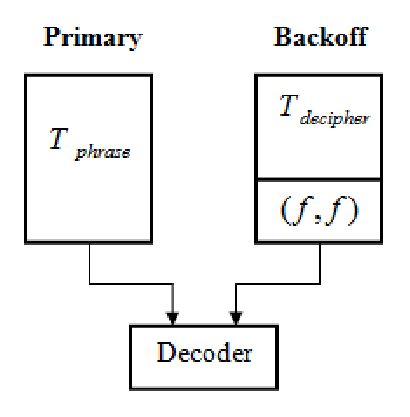
\includegraphics[width=1.8in,height=1.8in]{OOV}
%  \caption{A backoff model for improving OOV translations.}
%\label{backoff}
%\end{figure}



%For the same reason stated previously, we compare the following two systems against PBMT.

%\begin{itemize}
%\item Adj-OOV: Use $T_{decipher}$ learned from deciphering adjacent bigrams for translating OOV words.
%\item Dep-OOV: Use $T_{decipher}$ learned from deciphering typed dependency bigrams for translating OOV words.
%\end{itemize}
\subsubsection{A Combined Approach}
In the end, we build a system \textbf{Decipher-COMB}, which uses $T_{decipher}$ to improve translation of both observed and OOV words with methods described in sections \ref{d_obsv} and \ref{d_oov}.

\subsection{Results}
We tune each system three times with MERT and choose the best weights based on BLEU scores on tuning set.


 \begin{table*}[th]
 \begin{center}
 \begin{tabular}{ |c|c|c|c|c|c| } \hline
 Decipherment & System & $Tune_{2008}$ & $Test_{2009}$ & $Test_{2010}$ & $Test_{2011}$ \\ \hline
 None & PBMT (Baseline) &  19.1 & 19.6 & 21.3 & 22.1 \\ \hline \hline
   \multirow{3}{*}{Adjacent} & Decipher-OBSV &  19.5 & 20.1 & 22.2 & 22.6 \\ \hhline{~-----}
 &Decipher-OOV &  19.4 & 19.9& 21.7 & 22.5\\ \hhline{~-----}
 &Decipher-COMB &  19.5 & 20.2 & 22.3 & 22.5 \\ \hline \hline

  \multirow{3}{*}{Dependency} & Decipher-OBSV &19.7  & 20.5  & 22.5  & 23.0 \\ \hhline{~-----}
 & Decipher-OOV &  19.9  & 20.4 & 22.4  & 22.9 \\ \hhline{~-----}
 & Decipher-COMB &  20.0 & 20.8  & 23.1 & 23.4 \\ \hline


 \end{tabular}
 \caption{Systems that use translation lexicons learned from decipherment show consistent improvement over the baseline system across tuning and testing sets. The best system, Decipher-COMB, achieves as much as 1.8 BLEU point gain on the 2010 news test set.}
 \label{result}
 \end{center}
 \end{table*}

Table \ref{result} shows that the translation lexicon learned from decipherment helps achieve higher BLEU scores across tuning and testing sets. \textbf{Decipher-OBSV} improves BLEU scores by as much as 1.2 points. We analyze the results and find the gain mainly comes from two parts. First, adding $T_{decipher}$ to small amounts of parallel corpus improves word level translation probabilities, which lead to better lexical weighting; second, $T_{decipher}$ contains new alternative translations for words observed in the parallel corpus.

Moreover, \textbf{Decipher-OOV} also achieves better BLEU scores compared with PBMT across all tuning and test sets. We also observe that systems using $T_{decipher}$ learned by deciphering dependency bigrams leads to larger gains in BLEU scores. When decipherment is used to improve translation of both observed and OOV words, we see improvement in BLEU score as high as 1.8 points on the 2010 news test set.

The consistent improvement on the tuning and different testing data suggests that decipherment is capable of learning good translations for a number of OOV words. To further demonstrate that our decipherment approach finds useful translations for OOV words, we list the top 10 most frequent OOV words from both the tuning set and testing set as well as their translations (up to three most likely translations) in Table \ref{oov_translation}. $P(e|f)$ and $P(f|e)$ are average scores over different decipherment runs.

 \begin{table}
 \begin{center}
 \begin{tabular}{ |c|ccc|} \hline
Spanish & English & $P(e|f)$ & $P(f|e)$ \\ \hline
obama & his & 0.33 & 0.01 \\
           & bush & 0.27 & 0.07\\
           & clinton & 0.23 & 0.11 \\ \hline
bush & \textbf{bush} & 0.47 & 0.45 \\
        & yeltsin & 0.28 & 0.81 \\
        & he & 0.24 & 0.05 \\ \hline
festival & event & 0.68 & 0.35 \\
            &\textbf{festival} & 0.61 & 0.72 \\ \hline
wikileaks & zeta & 0.03 & 0.33 \\ \hline
venus & \textbf{venus} & 0.61 & 0.74 \\
          & serena & 0.47 & 0.62 \\ \hline
colchones & \textbf{mattresses} & 0.55 & 0.73 \\
                 & cars & 0.31 & 0.01 \\ \hline
helado & frigid & 0.52 & 0.44 \\
         & chill & 0.37 & 0.14 \\
           & sandwich & 0.42 & 0.27 \\ \hline
google & microsoft & 0.67 & 0.18 \\
            & \textbf{google} & 0.59 & 0.69 \\ \hline
cantante & \textbf{singer} & 0.44 & 0.92 \\
              & jackson & 0.14 & 0.33 \\
            & artists & 0.14 & 0.77 \\ \hline
mccain & \textbf{mccain} & 0.66 & 0.92 \\
            & it & 0.22 & 0.00 \\
            & he & 0.21 & 0.00 \\\hline
 \end{tabular}

 \caption{Decipherment finds correct translations for 7 out of 10 most frequent OOV word types.}
 \label{oov_translation}
 \end{center}
 \end{table}

From the table, we can see that decipherment finds correct translations (bolded) for 7 out of the 10 most frequent OOV words. Moreover, many OOVs and their correct translations are homographs , which makes copying OOVs directly to the output a strong baseline to beat. Nonetheless, decipherment still finds enough correct translations to improve the baseline.